\section{Suddivisione del lavoro}
Vengono qui di seguito descritti i ruoli ricoperti dai vari membri del gruppo durante lo svolgimento del progetto.
\subsection{Investimento non rendicontato}
\subsubsection{\AR}
Nel periodo di \AR{} ciascun componente dovrà ricoprire i seguenti ruoli e per la quantità di ore specificate:

\begin{table}[H]
	\centering
	\begin{tabular}{|l|c|c|c|c|c|c|c|}
		\hline
		\textbf{Nominativo} & 
		\multicolumn{6}{c|}{\textbf{Ore per ruolo}} & 
		\textbf{Ore totali} \\
		& Re & Am & An & Pj & Pr & Ve & \\
		\hline
		Nicola Dal Maso & & 7 & 10 & & & 10 & 27 \\
		Lorenzo Ferrarin & & 8 & 10 & & & 9 & 27 \\
		Beatrice Guerra & 15 & & 3 & & & 9 & 27 \\
		Marco Ponchia & & & 15 & & & 12 & 27 \\
		Tommaso Rosso & & 5 & 22 & & & & 27 \\
		Alice V. Sasso & & 9 & 18 & & & & 27 \\
		Mattia Zecchinato & 15 & & 12 & & & & 27 \\
		\hline
	\end{tabular}
	\caption{Ore per componente, periodo di \AR{}}
\end{table}
I valori sono riassunti nel seguente grafico, che rappresenta in maniera visiva per quante ore un membro ricoprirà un determinato ruolo.
\begin{figure}[H]
	\centering
	\includegraphics[width=14cm]{img_suddlavoro/AA.png}
	\caption{Ore per componente, periodo di \AR{}}
\end{figure}

\subsection{Investimento rendicontato}
\subsubsection{\AD}
Nel periodo di \AD{} ciascun componente dovrà ricoprire i seguenti ruoli e per la quantità di ore specificate:

\begin{table}[H]
	\centering
	\begin{tabular}{|l|c|c|c|c|c|c|c|}
		\hline
		\textbf{Nominativo} & 
		\multicolumn{6}{c|}{\textbf{Ore per ruolo}} & 
		\textbf{Ore totali} \\
		& Re & Am & An & Pj & Pr & Ve & \\
		\hline
		Nicola Dal Maso & & & 3 & & &  & 3 \\
		Lorenzo Ferrarin & & 1 & 2 & & &  & 3 \\
		Beatrice Guerra & & & 1 & & & 2 & 3 \\
		Marco Ponchia & & & 1 & & & 2 & 3 \\
		Tommaso Rosso & & 3 & & & & & 3 \\
		Alice V. Sasso & & & 3 & & & & 3 \\
		Mattia Zecchinato & 1 & & 2 & & & & 3 \\
		\hline
	\end{tabular}
	\caption{Ore per componente, periodo di \AD}
\end{table}
I valori sono riassunti nel seguente grafico, che rappresenta in maniera visiva per quante ore un membro ricoprirà un determinato ruolo.
\begin{figure}[H]
	\centering
	\includegraphics[width=14cm]{img_suddlavoro/AD.png}
	\caption{Ore per componente, periodo di \AD{}}
\end{figure}

\subsubsection{\PA}
Nella periodo di \PA{} ciascun componente dovrà ricoprire i seguenti ruoli e per la quantità di ore specificate:

\begin{table}[H]
	\centering
	\begin{tabular}{|l|c|c|c|c|c|c|c|}
		\hline
		\textbf{Nominativo} & 
		\multicolumn{6}{c|}{\textbf{Ore per ruolo}} & 
		\textbf{Ore totali} \\
		& Re & Am & An & Pj & Pr & Ve & \\
		\hline
		Nicola Dal Maso &4 & &3 &20 & & & 27 \\
		Lorenzo Ferrarin & & &2 &15 & &10 & 27 \\
		Beatrice Guerra & & &4 &14 & &10 & 28 \\
		Marco Ponchia & &4 &8 &15 & & & 27 \\
		Tommaso Rosso & &2 & &9 & &15 & 26 \\
		Alice V. Sasso &4 & &4 &20 & & & 28 \\
		Mattia Zecchinato & & &2 &8 & &20 & 30 \\
		\hline
	\end{tabular}
	\caption{Ore per componente, periodo di \PA{}}
\end{table}
I valori sono riassunti nel seguente grafico, che rappresenta in maniera visiva per quante ore un membro ricoprirà un determinato ruolo.
\begin{figure}[H]
	\centering
	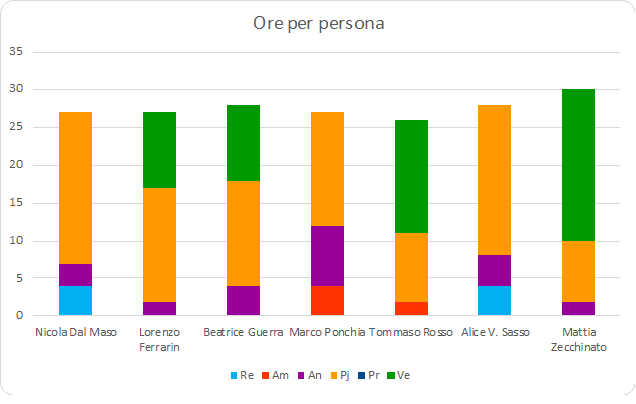
\includegraphics[width=14cm]{img_suddlavoro/PA.png}
	\caption{Ore per componente, periodo di \PA{}}
\end{figure}

\subsubsection{\PD}
Nel periodo di \PD{} ciascun componente dovrà ricoprire i seguenti ruoli e per la quantità di ore specificate:

\begin{table}[H]
	\centering
	\begin{tabular}{|l|c|c|c|c|c|c|c|}
		\hline
		\textbf{Nominativo} & 
		\multicolumn{6}{c|}{\textbf{Ore per ruolo}} & 
		\textbf{Ore totali} \\
		& Re & Am & An & Pj & Pr & Ve & \\
		\hline
		Nicola Dal Maso & & & &12 & &14 & 26 \\
		Lorenzo Ferrarin &5 & &2 &14 & & & 21 \\
		Beatrice Guerra & &4 & &19 & & & 23 \\
		Marco Ponchia &3 & & &19 & & & 22 \\
		Tommaso Rosso & & &2 &14 & &8 & 24 \\
		Alice V. Sasso & & & &10 & &14 & 24 \\
		Mattia Zecchinato & &4 & &19 & & & 23 \\
		\hline
	\end{tabular}
	\caption{Ore per componente, periodo di \PD{}}
\end{table}
I valori sono riassunti nel seguente grafico, che rappresenta in maniera visiva per quante ore un membro ricoprirà un determinato ruolo.
\begin{figure}[H]
	\centering
	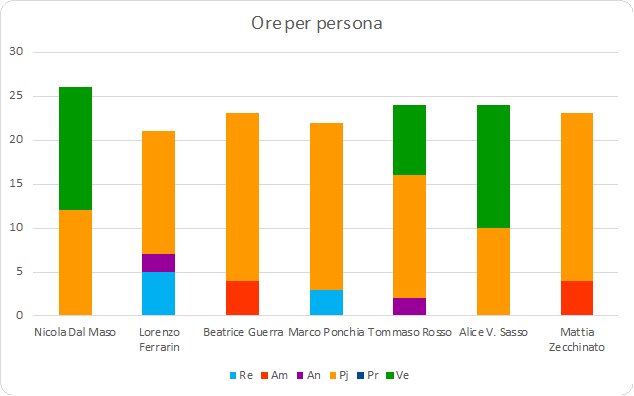
\includegraphics[width=14cm]{img_suddlavoro/PD2.png}
	\caption{Ore per componente, periodo di \PD{}}
\end{figure}

\subsubsection{\Cod}
Nel periodo di \Cod{} ciascun componente dovrà ricoprire i seguenti ruoli e per la quantità di ore specificate:

\begin{table}[H]
	\centering
	\begin{tabular}{|l|c|c|c|c|c|c|c|}
		\hline
		\textbf{Nominativo} & 
		\multicolumn{6}{c|}{\textbf{Ore per ruolo}} & 
		\textbf{Ore totali} \\
		& Re & Am & An & Pj & Pr & Ve & \\
		\hline
		Nicola Dal Maso &4 & & & &26 & & 30 \\
		Lorenzo Ferrarin & & & &5 &21 &10 & 36 \\
		Beatrice Guerra & & & & &24 &9 & 33 \\
		Marco Ponchia & &4 & & &12 &18 & 34 \\
		Tommaso Rosso &5 & & &6 &24 & & 35 \\
		Alice V. Sasso & & & & &14 &18 & 32 \\
		Mattia Zecchinato & & & &5 &26 & & 31 \\
		\hline
	\end{tabular}
	\caption{Ore per componente, periodo di \Cod{}}
\end{table}
I valori sono riassunti nel seguente grafico, che rappresenta in maniera visiva per quante ore un membro ricoprirà un determinato ruolo.
\begin{figure}[H]
	\centering
	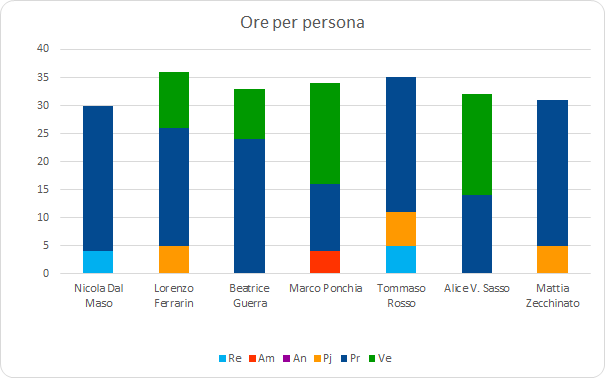
\includegraphics[width=14cm]{img_suddlavoro/C2.png}
	\caption{Ore per componente, periodo di \Cod{}}
\end{figure}

\subsubsection{\VV}
Nel periodo di \VV{} ciascun componente dovrà ricoprire i seguenti ruoli e per la quantità di ore specificate:

\begin{table}[H]
	\centering
	\begin{tabular}{|l|c|c|c|c|c|c|c|}
		\hline
		\textbf{Nominativo} & 
		\multicolumn{6}{c|}{\textbf{Ore per ruolo}} & 
		\textbf{Ore totali} \\
		& Re & Am & An & Pj & Pr & Ve & \\
		\hline
		Nicola Dal Maso & &5 & &6 & &9 & 20 \\
		Lorenzo Ferrarin & &5 & &3 & &11 & 19 \\
		Beatrice Guerra &5 & & & & &14 & 19 \\
		Marco Ponchia & & & & &8 &12 & 20 \\
		Tommaso Rosso & & & &4 &4 &10 & 18 \\
		Alice V. Sasso & &6 & & & &13 & 19 \\
		Mattia Zecchinato &5 & & & & &14 & 19 \\
		\hline
	\end{tabular}
	\caption{Ore per componente, periodo di \VV{}}
\end{table}
I valori sono riassunti nel seguente grafico, che rappresenta in maniera visiva per quante ore un membro ricoprirà un determinato ruolo.
\begin{figure}[H]
	\centering
	\includegraphics[width=14cm]{img_suddlavoro/VV.png}
	\caption{Ore per componente, periodo di \VV{}}
\end{figure}

\subsection{Totale}
\subsubsection{Ore totali con investimento}
Le ore totali, comprese quelle investite in analisi, divise per componente durante il progetto saranno le seguenti:

\begin{table}[H]
	\centering
	\begin{tabular}{|l|c|c|c|c|c|c|c|}
		\hline
		\textbf{Nominativo} & 
		\multicolumn{6}{c|}{\textbf{Ore per ruolo}} & 
		\textbf{Ore totali} \\
		& Re & Am & An & Pj & Pr & Ve & \\
		\hline
		Nicola Dal Maso &8 &12 &16 &38 &26 &33 & 133 \\
		Lorenzo Ferrarin &5 &14 &16 &37 &21 &40 & 133 \\
		Beatrice Guerra &20 &4 &8 &33 &24 &44 & 133 \\
		Marco Ponchia &3 &8 &24 &34 &20 &44 & 133 \\
		Tommaso Rosso &5 &7 &27 &33 &28 &33 & 133 \\
		Alice V. Sasso &4 &15 &25 &30 &14 &45 & 133 \\
		Mattia Zecchinato &21 &4 &16 &32 &26 &34 & 133 \\
		\hline
	\end{tabular}
	\caption{Ore totali per componente compresa l'analisi non rendicontata}
\end{table}
%I valori sono riassunti nel seguente grafico, che rappresenta in maniera visiva per quante ore un membro ricoprirà un determinato ruolo.
%\begin{figure}[H]
%	\centering
%	\includegraphics[width=14cm]{img_suddlavoro/TOT.png}
%	\caption{Ore totali per componente}
%\end{figure}

\subsubsection{Ore totali senza investimento}
Le ore totali rendicontate, cioè quelle senza investimento iniziale, divise per componente durante il progetto saranno le seguenti:

\begin{table}[H]
	\centering
	\begin{tabular}{|l|c|c|c|c|c|c|c|}
		\hline
		\textbf{Nominativo} & 
		\multicolumn{6}{c|}{\textbf{Ore per ruolo}} & 
		\textbf{Ore totali} \\
		& Re & Am & An & Pj & Pr & Ve & \\
		\hline
		Nicola Dal Maso &8 &5 &3 &38 &26 &23 & 103 \\
		Lorenzo Ferrarin &5 &5 &4 &37 &21 &31 & 103 \\
		Beatrice Guerra &5 &4 &4 &33 &24 &33 & 103 \\
		Marco Ponchia &3 &8 &8 &34 &20 &30 & 103 \\
		Tommaso Rosso &5 &2 &2 &33 &28 &33 & 103 \\
		Alice V. Sasso &4 &6 &4 &30 &14 &45 & 103 \\
		Mattia Zecchinato &5 &4 &2 &32 &26 &34 & 103 \\
		\hline
	\end{tabular}
	\caption{Ore totali rendicontate senza investimento iniziale}
\end{table}
I valori sono riassunti nel seguente grafico, che rappresenta in maniera visiva per quante ore un membro ricoprirà un determinato ruolo.
\begin{figure}[H]
	\centering
	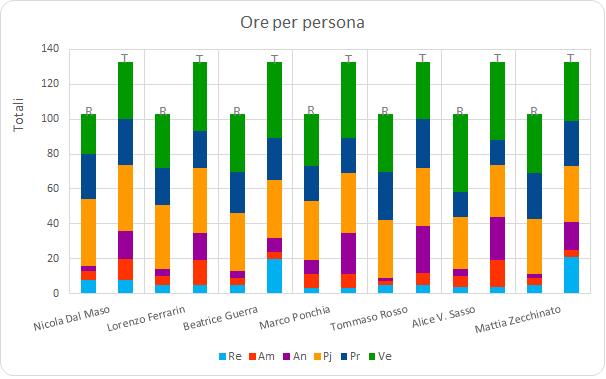
\includegraphics[width=14cm]{img_suddlavoro/TOT2.png}
	\caption{Ore totali per componente}
\end{figure}





